\documentclass[main.tex]{subfiles}

\begin{document}

% \textcolor{red}{Вводная лекция}

\section{Лекция 11.05.2021 (Байкин А.Н.)}

\subsection{Моделирование течения жидкости в скважине}

Мы с вами движемся дальше.
Сегодня у нас будет тема про моделирование скважин.
Т.е. до этого мы рассматривали преимущественно именно процессы в самой трещине, процессы в окружающем пласте (такие как утечки или деформация породы), а закачка всегда предполагалась на забое скважины (расход задавался на входе в саму трещину).
Но вообще говоря у нас с вами есть скважины и то давление на входе в трещину, которое мы получаем в расчётах, не совпадает с давлением, которое мы получаем при измерении какими-то приборами (как на поверхности, так и когда мы опускаем датчик давления вниз к забою).
\\

\subsubsection{Зачем моделировать скважину?}

\includegraphics[width=\textwidth, page=65]{HF_slides_2022.pdf}

Зачем нам необходимо моделировать скважину?

Во-первых, чтобы знать, какое давление на забое скважины и как оно соотносится с давлением на устье скважины.
Почему это важно?
С одной стороны, можно было бы сказать: давайте поставим датчик давления на забое и всё будет классно, но этот датчик давления будет стоять не на самой трещине (т.е. между датчиком и трещиной будет либо участок трубы, либо как минимум участки перфорации, вдоль которых возникает падение давления из-за трения; в итоге, измеряемое давление BHP будет немного выше, чем давление на входе в трещину).
Датчик забойного давления BHP (забойный манометр) практически никогда не ставят, потому что это дорого; обычно мы знаем только давление на устье WHP.

Чтобы осуществить пересчёт BHP через известное WHP нам необходимо учесть падение давления за счёт трения жидкости при движении по трубе и гидростатическое давление.
Т.е. получаем, что за счёт трения давление на забое снижается (относительно WHP), а за счёт гидростатики давление на забое увеличивается (относительно WHP).

Кроме того, скважину интересно моделировать, чтобы объяснить наблюдаемый hammer effect: при резком закрытии скважины наблюдаются колебательные движения жидкости между скважиной и трещиной, которые имеют форму затухающих колебаний.
И по этим затухающим колебаниям пытаются проводить диагностику. Как минимум говорят, что если есть hammer effect, то связь между скважиной и трещиной достаточно хорошая (т.е. перфорацию сделали достаточно качественно).
Дальше по hammer эффекту пытаются оценить размеры трещины (ширину, длину).

Ещё дальше пытаются понять, какой порт заработал (если есть несколько портов) -- правда это уже немного другая технология, которая называется tube waves от компании Schlumberger.
\\

\includegraphics[width=\textwidth, page=66]{HF_slides_2022.pdf}

Для чего ещё моделировать скважину?

Если мы запустили пульсы проппанта (с определённой концентрацией) наверху (на устье), то никто не говорит, что они в таком же первозданном виде дойдут до забоя.
Вообще говоря, они могут размазаться.

Сегодня мы размазывание не будем рассматривать, потому что для этого нужна двухскоростная модель, а сегодня мы рассмотрим только односкоростную модель.
Но вообще говоря из-за того, что у нас есть профиль скорости, частички проппанта будут собираться (проваливаться) к центру.

Также может происходить оседание проппанта.
В принципе всё, что происходило с проппантом в трещине (например, оседание), верно и для скважины.
 
Размазывание концентрации проппанта важно моделировать, чтобы понимать, какое значение концентрации будет на входе в трещину.

\underline{Замечание аудитории.}
Слышали, что при движении по круглой трубе частички проппанта будут собираться в кольцо на расстоянии 0.6 радиуса от центра.
Говорят, что это связано с тем, что сами частички проппанта могут крутиться вокруг своей оси.


Сегодня рассмотрим модель попроще, чтобы вы поняли общую схему, а дальше уже можно придумывать более сложные модели (главное понять, какой эффект хочется описать).
\\

\subsubsection{Предположения модели}

\includegraphics[width=\textwidth, page=67]{HF_slides_2022.pdf}

Теперь давайте приступим к самой модели.

Основные предположения модели:

1) наклонная скважина переменного радиуса $R$ (на рисунке я специально нарисовал 2 цилиндра, т.к. скважина, вообще говоря, может иметь переменное сечение, но в реальности оно обычно кусочно постоянное: берут кусок трубы одного диаметра засовывают, дальше другого диаметра, дальше обсадная колонна и так далее);

2) односкоростная модель $\vec{u}_p=\vec{u}_f=\vec{u}_m$ (жидкость и проппант движутся с одинаковой скоростью и эта скорость равна усреднённой скорости, формула для которой была в прошлый раз) -- это оправдано, когда жидкость достаточно вязкая и частички проппанта как-бы заморожены в жидкость;

3) жидкость неньютоновская (т.е. жидкость со степенной реологией);

4) течение не расслаивается (не может быть такого, что где-то на горизонтальном участке проппант внизу пошёл (полностью осел) и течение расслоилось);

5) ламинарный, переходный, турбулентный режимы;

6) сжимаемостью жидкости пренебрегаем.
\\

\subsubsection{Определяющие уравнения}

\includegraphics[width=\textwidth, page=68]{HF_slides_2022.pdf}

Что нам нужно, чтобы описать течение рассматриваемой жидкости?

1) Закон сохранения объёма проппанта:
\beq\label{ZSM_proppant}
\frac{\partial\left(cS(x)\right)}{\partial t}+\frac{\partial\left(cS(x)u_p\right)}{\partial x}=0,\,\,\,\,\,c_p\equiv c
\eeq

2) Закон сохранения объёма жидкости:
\beq\label{ZSM_fluid}
\frac{\partial\left((1-c)S(x)\right)}{\partial t}+\frac{\partial\left((1-c)S(x)u_f\right)}{\partial x}=0,\,\,\,\,\,c_f\equiv 1-c
\eeq

Уравнения \eqref{ZSM_proppant} и \eqref{ZSM_fluid} уже усреднённые по сечению скважины, но они выводятся точно также, как и для течения проппанта в трещине (только сейчас вместо раскрытия трещины $w(x)$ используем площадь сечения $S(x)$ и сейчас нет утечек).

Далее используя предположение односкоростной модели $u_p=u_f=u_m$, где $u_m$ -- среднеобъёмная усреднённая скорость смеси по сечению $S(x)$, складываем уравнения \eqref{ZSM_proppant} и \eqref{ZSM_fluid} (дополнительно учтём, что производная площади сечения по времени равна нулю):
\beq\label{Q_const_t}
\frac{\partial\left(S(x)u_m\right)}{\partial x}=\frac{\partial\left(Q(t,x)\right)}{\partial x}=0,
\eeq
где $Q(t,x)=Su_m=const(t)=Q_{inlet}(t),\,\,\,\,S=\pi R^2$.

Полученное уравнение говорит нам о том, что расход через любое поперечное сечение скважины одинаков (нет зависимости расхода от координаты $x$) и зависит от расхода, закачиваемого в скважину сверху.
Если изменяется сечение скважины, то соответственно изменяется скорость течения так, чтобы расход оставался прежним.

3) Граничное условие (на концентрацию проппанта) на устье скважины:
\beq\label{proppant_concentration_gu}
c|_{x=0}=c_{inlet}(t)
\eeq

Если проводить аналогию с течением проппанта в трещине, то уравнение \eqref{Q_const_t} аналогично эллиптическому уравнению, в котором необходимо было искать давление.

В итоге: мы знаем расход $Q_{inlet}(t)$; знаем площадь $S(x)$; можем найти скорость $u_m(x,t)$; как только знаем скорость, мы можем подставить её в уравнение \eqref{ZSM_proppant}, решить это уравнение и с учётом граничного условия \eqref{proppant_concentration_gu} найти концентрацию проппанта.
\\

При решении данной задачи можно использовать тот же алгоритм, что и для переноса проппанта в трещине, т.е. взять одномерную разностную схему (например, Лакса-Вендроффа с лимитерами), но я хотел бы ещё показать другой численный алгоритм.
В данном случае, когда рассматриваем односкоростную модель, этот алгоритм проще, намного быстрее и точнее.
\\

\subsubsection{Численный алгоритм}

\includegraphics[width=\textwidth, page=69]{HF_slides_2022.pdf}

Можно показать, что в случае односкоростной модели уравнение \eqref{ZSM_proppant} для переноса проппанта можно переписать в более простом виде:
\beq\label{ProppantTransfer}
\frac{\partial c}{\partial t}+u_m\frac{\partial c}{\partial x}=0
\eeq
(уравнение \eqref{ZSM_proppant} -- это закон сохранения в дивергентной форме; а уравнение \eqref{ProppantTransfer} -- это классическое уравнение переноса, которое всем известно с урматов).

Физический смысл уравнения \eqref{ProppantTransfer}: концентрация $c$ неизменно переносится векторным полем $\vec{u}$ (в данном случае со скоростью $u_m$ вдоль скважины).

Опять же мы здесь должны сделать (ввести) дискретизацию по времени.
Разобьём суммарное время закачки на $k-1$ временных интервалов:
\beq
\Delta t_k=t_k-t_{k-1},\,\,\,\,\,t_0=0
\eeq

Введём вспомогательное обозначение: $F_k$ -- это значение величины $F$ в момент времени $t_k$.

В Лагранжевых координатах $(t,X)$ на интервале $[t_k, t_{k+1}]$ имеем решение вида:
\beq\label{LagrangePosition}
c(t,X(t))=c(t,X|_{t=t_k}),\,\,\,\,\,X(t)=X|_{t=t_k}+\int\limits_{t_k}^{t}u_m(X(s))ds
\eeq

Грубо говоря, мы в начале трубы выпускаем некоторую лагранжеву частицу со скоростью $u_m$, и формула \eqref{LagrangePosition} говорит нам, что эта частица через время $t$ дойдёт до положения с координатой $X$.
И соответственно, если $c$ на входе будет постоянным, то концентрация за рассматриваемое время тоже не изменится.

\includegraphics[width=\textwidth, page=70]{HF_slides_2022.pdf}

Соответственно мы можем рассматривать весь этот процесс в виде набора фронтов концентрации.
За каждый новый шаг по времени мы выпускаем новый фронт, далее он движется по трубе и мы фиксируем кусочно постоянный уровень концентрации проппанта на каком-то участке скважины.

Чтобы перейти в Эйлерову сетку в точке $x$, мы просто смотрим между какими фронтами эта точка $x$ лежит и говорим, что концентрация равна этому значению.
\\
Здесь (для односкоростной модели) всё достаточно просто и можно обойтись решением обыкновенных дифференциальных уравнений для концентрации проппанта.

\includegraphics[width=\textwidth, page=71]{HF_slides_2022.pdf}

Нам нужна не только концентрация, а прежде всего нам нужно знать давление.
Если на забое будет слишком большое давление, то жидкость может просто порвать трубу.
Как будем считать давление?
Для этого берём уравнение Навье-Стокса.
Выводим аналогично выводу транспорта проппанта для трещины.
Но здесь в роли малого параметра будет
$$\varepsilon=\frac{2R}{L},$$
где $2R$ -- диаметр скважины; $L$ -- длина скважины (диаметр скважины порядка 10 см, а длина скважины порядка 1 км -- ясно, что параметр $\varepsilon$ будет достаточно малым и можно использовать приближение тонкого слоя, но уже в цилиндрической геометрии).

Вдоль оси $Ox$ (ось направлена вдоль скважины; $\theta$ -- угол между осью скважины и поверхностью Земли; $\tau$ -- тензор вязких напряжений):
\beq\label{NavieOx}
0=-\frac{dp(x)}{dx}+\frac{1}{r}\frac{d}{dr}\left(r\tau_{rx}\right)+\rho g\sin\theta
\eeq

В случае ньютоновской жидкости:
\beq\label{TauRX}
\tau_{ij}=2\mu_sD_{ij},\,\,\,\,\,D=\frac{1}{2}\left(\nabla u + (\nabla u)^T\right),\,\,\,\,\,\tau_{rx}=\mu_s\frac{\partial u_x}{\partial r}.
\eeq
(в приближении тонкого слоя можно показать, что будет всего одна компонента $\tau_{rx}$)

Кроме того, есть зависимость вязкости смеси от концентрации проппанта.
Формула Нолти:
\beq
\mu_s(c)=\mu_f\left(1-\frac{c}{c_{max}}\right)^{-2.5n_{clean}},
\eeq
где $c_{max}=0.65$ -- максимальная концентрация упаковки проппанта, $\mu_f$ -- вязкость чистой жидкости (гель без проппанта), $n_{clean}$ -- индекс течения (один из реологических параметров) чистой жидкости (без проппанта).

В случае неньютоновской жидкости по формуле Нолти будет изменяться не вязкость, а реологический параметр $K$.

\includegraphics[width=\textwidth, page=72]{HF_slides_2022.pdf}

Первоначальная наша задача: вывести вид профиля скорости.
По сути сейчас докажем формулу для течения Пуазейля с учётом силы тяжести.

Подставим \eqref{TauRX} для $\tau_{rx}$ в \eqref{NavieOx}:

\beq
0=-\frac{dp(x)}{dx}+\frac{1}{r}\frac{d}{dr}\left(r\mu_s\frac{\partial u_x}{\partial r}\right)+\rho g \sin{\theta}
\eeq

Домножим на $r$:
\beq
\frac{d}{dr}\left(r\mu_s\frac{\partial u_x}{\partial r}\right)=\left(\frac{dp(x)}{dx}-\rho g\sin{\theta}\right)r
\eeq

Интегрируем с учётом $\tau_{rx}|_{r=0}=0$ (условие регулярности):
\beq
\mu_s\frac{\partial u_x}{\partial r}=\left(\frac{dp}{dx}-\rho g\sin{\theta}\right)\frac{r}{2}
\eeq

Интегрируем ещё раз:
\beq
u_x(r)=\frac{1}{4\mu_s}\left(\frac{dp}{dx}-\rho g\sin{\theta}\right)r^2+C
\eeq

Используя граничное условие $u_x|_{r=R}=0$ (условие прилипания на границе), находим константу $C$.
Получаем:
\beq
u_x(r)=\underbrace{-\frac{R^2}{4\mu_s}\left(\frac{dp}{dx}-\rho g\sin{\theta}\right)}_{u_{max}}\left(1-\frac{r^2}{R^2}\right)=u_{max}\left(1-\frac{r^2}{R^2}\right)
\eeq

Максимальная скорость $u_{max}$ достигается при $r=0$.

\subsubsection{Вычисление средней скорости}

\includegraphics[width=\textwidth, page=73]{HF_slides_2022.pdf}

Нашли максимальную скорость $u_{max}$, а уравнение переноса записано в терминах средней скорости, поэтому необходимо найти соотношение между средней скоростью и максимальной скоростью.

Возьмём и усредним найденный профиль скорости по сечению (сделаем в полярных координатах, т.е. якобиан $r$):
\begin{multline}
u_m=\frac{1}{|S|}\int\limits_S{u_xdS}=\frac{1}{\pi R^2}\int\limits_{0}^{2\pi}\int\limits_{0}^{R}u_{max}r\left(1-\frac{r^2}{R^2}\right)drd\varphi=\\=u_{max}\frac{2\pi}{\pi}\int\limits_0^1\frac{r}{R}\left(1-\frac{r^2}{R^2}\right)d\left(\frac{r}{R}\right)=\frac{u_{max}}{2}
\end{multline}

Таким образом, получаем среднюю скорость ламинарного течения:
\beq
u_m=-\frac{R^2}{8\mu_s}\left(\frac{dp}{dx}-\rho g\sin{\theta}\right)
\eeq

В целом отсюда можно найти давление для ламинарного течения!
Интегрируем по $x$ (по оси скважины).
$\theta$ может меняться, $\rho$ может меняться, $R$ может меняться, вязкость $\mu_s$ зависит от концентрации, $u_m$ тоже меняется в зависимости от сечения.
Соответственно берём интегрируем и отсюда находим давление $p(x)$.
Но мы поступим немного по-другому.

\subsubsection{Средняя скорость для степенной жидкости}

\includegraphics[width=\textwidth, page=74]{HF_slides_2022.pdf}

В тех же самых предположениях можем вывести профиль скорости для степенной жидкости:
\beq
\tau_{ij}=K_s\dot{\gamma}^{n-1}D_{ij},\,\,\,\,\,\dot{\gamma}=\sqrt{\frac{1}{2}\sum\limits_{i,j=1}^{3}D_{ij}^2}
\eeq
Профиль скорости:
\beq
u_x=u_{max}\left(1-\left(\frac{r}{R}\right)^{(n+1)/n}\right)
\eeq
\ \\

\subsubsection{Коэффициент трения Фаннинга для ламинарного и турбулентного течений}

\includegraphics[width=\textwidth, page=75]{HF_slides_2022.pdf}

Сейчас выведем формулу для давления немного по-другому.
Опять стартуем с уравнения Навье-Стокса и сразу усредняем (по площади):
\beq
0=-\frac{dp(x)}{dx}+\frac{1}{r}\frac{d}{dr}\left(r\tau_{rx}\right)+\rho g \sin{\theta}\,\,\bigg|\,\,\,\,\,\frac{1}{\pi R^2}\int\limits_S(\cdot)dS
\eeq

Получаем следующее уравнение ($\overline{p}$ на самом деле можно заменить на просто $p$, так как мы знаем, что давление выравнивается вдоль сечения -- это можно доказать в предположениях течения тонкого слоя):
\beq\label{PressureGeneral}
\frac{d\overline{p}}{dx}=-\frac{2\tau_w}{R}+\overline{\rho}g\sin{\theta},
\eeq
где $\tau_w=-\tau_{rx}|_{r=R}$ -- напряжение сдвига (трения) на стенке трубы.
Его можно измерить при ламинарном течении, а также и в случае турбулентного течения (например, для известного перепада давления найти $\tau_w$ из \eqref{PressureGeneral} -- т.е. решить обратную задачу), поэтому этот вывод формулы для давления более общий (в предыдущем выводе не понятно, что такое профиль скорости в случае турбулентного течения).

Видим, что для определения давления профиль скорости нам и не нужен.
Можем найти давление, если известен $\tau_w$ (находим давление просто проинтегрировав уравнение \eqref{PressureGeneral}).

Обычно экспериментаторы работают с безразмерными величинами для того, чтобы можно было масштабировать результаты (измерить на одной трубе, а распространить результаты на трубы произвольного диаметра), поэтому вводят коэффициент трения Фаннинга:
\beq
f_s=\frac{\tau_w}{\rho u_m^2/2}
\eeq

Тогда уравнение \eqref{PressureGeneral} примет вид:
\beq
\frac{dp}{dx}=-\frac{\rho u_m^2}{R}f_s+\rho g\sin{\theta}
\eeq

Какой физический смысл у полученного уравнения?
Это баланс сил: есть сила давления, кроме того проталкивать жидкость нам помогает сила тяжести, а препятствует трение жидкости о стенки трубы.
Поэтому можно вывести уравнение \eqref{PressureGeneral} другим способом, а именно просто расписать баланс сил:

силы трения $\tau_w\cdot2\pi R\cdot L$;

силы прикладываемого давления $\left(p_1-p_2\right)S$

силы тяжести $\rho g\sin{\theta} \cdot S\cdot L$

Получим:
\beq
\left(p_2-p_1\right)S+\rho g\sin{\theta} \cdot S\cdot L-\tau_w\cdot2\pi R\cdot L=0
\eeq
разделим обе части на $S\cdot L$:
\beq
\frac{p_1-p_2}{L}+\rho g\sin{\theta}-\tau_w\cdot\frac{2\pi R}{\pi R^2}=0
\eeq
равносильно
\beq
\frac{p_2-p_1}{L}=\rho g\sin{\theta}-\frac{2\tau_w}{R},
\eeq
что и требовалось показать.
\\

\includegraphics[width=\textwidth, page=76]{HF_slides_2022.pdf}

Давайте найдём коэффициент Фаннинга для ламинарного течения.

Профиль скорости:
\beq
u_x=2u_m\left(1-\left(\frac{r}{R}\right)^2\right)
\eeq

Подставляем профиль скорости в выражение для $\tau_w$:
\beq
\tau_w=-\mu_s\frac{\partial u_x}{\partial r}\bigg|_{r=R}=\frac{4\mu_s u_m}{R}
\eeq

Подставляем $\tau_w$ в выражение для коэффициента Фаннинга:
\beq
f_s=\frac{\tau_w}{\rho u_m^2/2}=\frac{4\mu_s u_m}{R\rho u_m^2/2}=\frac{8\cdot 2}{\rho u_m(2R)/\mu_s}=\frac{16}{Re},
\eeq
где
$$Re=\frac{\rho u_m(2R)}{\mu_s}\text{ -- число Рейнольдса}$$

Для степенной жидкости можно показать, что
\beq
f_s=\frac{16}{Re'},
\eeq
где
$$Re'=\dfrac{\rho u_m^{2-n}(2R)^n}{K_s\left(\dfrac{3n+1}{4n}\right)^n8^{n-1}}-\text{обобщённое число Рейнольдса}$$

\includegraphics[width=\textwidth, page=77]{HF_slides_2022.pdf}

Для турбулентного течения явной формулы для коэффициента Фаннинга нет, но есть экспериментальные корреляции.
Эти экспериментальные корреляции записаны в неявном виде.
Есть разные корреляции как для ньютоновской, так и для неньютоновской жидкостей.
Коэффициенты в корреляциях могут зависеть от шероховатости трубы.
Обычно в корреляциях дополнительно присутствуют число Рейнольдса и реологический параметр жидкости $n$.

Из неявных корреляций можно приближённо выразить коэффициент трения Фаннинга $f_s$.

\includegraphics[width=\textwidth, page=78]{HF_slides_2022.pdf}

Почему у корреляции с предыдущего слайды именно такой вид?
Откуда взялся логарифм?

Есть так называемая двухслойная модель турбулентности.
О чём она нам говорит?
Вблизи стенки трубы скорости маленькие, соответственно число Рейнольдса небольшое и будет слой, в котором преимущественно ламинарное течение.
А в центре, где влияние вязкости небольшое (а скорость большая) имеется турбулентное ядро.

По так называемой модели фон Кармана сдвиг скорости обратно пропорционален расстоянию от стенки:
\beq
\frac{\partial u_x}{\partial y}=\frac{u^*}{\kappa y}
\eeq
Иначе говоря, если вводить турбулентную вязкость (или турбулентную диффузию), то она будет пропорциональна $y$.

Соответственно при интегрировании этого уравнения и получается логарифм с неопределёнными коэффициентами, значения которых определяются с помощью подгонки к экспериментальным данным.

Здесь не буду сильно останавливаться.
Просто, чтобы вы на пальцах понимали, откуда здесь внезапно появился логарифм.

\includegraphics[width=\textwidth, page=79]{HF_slides_2022.pdf}

Итак, у нас есть ламинарный коэффициент трения Фаннинга и есть турбулентный коэффициент трения Фаннинга.
А что в промежутке?

В промежутке задана линейная интерполяция в логарифмических координатах.

Откуда эта линейная интерполяция была получена?
Из экспериментов были получены критические значения числа Рейнольдса при переходе в разные режимы.
На графике видим хорошее совпадение с экспериментальными данными.

\subsubsection{Расчёт давления}

\includegraphics[width=\textwidth, page=80]{HF_slides_2022.pdf}

Теперь давайте перейдём к самому расчёту давления.
У нас есть градиент давления, который равен гидростатике минус трение (грубо говоря):
\beq
\frac{d\overline{p}}{dx}=-\frac{2\tau_w}{R}+\overline{\rho}g\sin{\theta}
\eeq

Если проинтегрировать по всей скважине, то мы получим, что давление на забое есть давление на устье плюс гидростатика  минус падение давления за счёт трения о стенку трубы.
\beq
p_{bh}(t,x)=p_{wh}(t)+\Delta p_h(t,x)-\Delta p_{fric}(t,x)
\eeq

Гидростатика:
\beq
\Delta p_h(t,x)=\int\limits_{0}^{x}\rho_s(c(t,s))g\,\sin{\theta(s)}ds
\eeq

\beq
\rho_s(c)=\rho_p c+\rho_f\left(1-c\right)
\eeq

Трение:
\beq
\Delta p_{fric}(t,x)=\int\limits_0^x\frac{2\tau_w(t,s)}{R(s)}ds - \text{давление трения}
\eeq

\includegraphics[width=\textwidth, page=81]{HF_slides_2022.pdf}

Хотел бы показать сравнение с полевыми данными.
Мы построили односкоростную модель, которая включает в себя уравнение переноса и формулу для давления.

Здесь мы будем сравнивать давления: $p_f^{ref}$ -- давление трения экспериментальное, $p_h^{ref}$ -- давление гидростатическое экспериментальное.
Видно, что гидростатическое давление хорошо подгоняется под экспериментальные данные, а с давлением трения есть некоторые проблемы.
Почему эти проблемы могут возникать и как их можно исправить?
На левом графике видно, что в начале давление трения  в модели падает, а по полевым данным растёт.
А на следующем участке завышено давление трения в модели.

Здесь сразу опишу ситуацию: здесь закачивалось несколько жидкостей.
Как мы исправили эту ситуацию?
Мы меняли свойства жидкости.
На правом графике поставили вторую жидкость и получилось лучшее совпадение с полевыми данными.
Плюс немного играли с корреляциями: можно использовать формулу Nolte, а можно использовать формулу Keck и таким образом подбивать (калибровка корреляции может дать более адекватный результат).

Кстати, то что жидкость не та качается (реологические параметры $K$ и $n$ другие) -- это нормальная ситуация, ведь то, что забрасывается в трубу не совпадает с тем, что указано в паспорте, потому что во-первых гель может не успеть сшиться (и тогда трения совсем другие будут, т.к. $K$ и $n$ разные у сшитого и несшитого геля), а во-вторых невозможно узнать все условия проведения полевого эксперимента (в лучшем случае нам дают графики давления и полевой отчёт, в котором представлено расписание закачки и т.д.)

На практике инженеры используют не корреляции для коэффициента трения Фаннинга, а у них уже есть таблицы с величиной градиента давления трения ($-2\tau_w/R$) для различных диаметров трубы и различных расходов жидкости.

Из step-down теста, постепенно снижая расход и смотря, как падает давление, можно посчитать коэффициент трения Фаннинга в трубе.

Обычно это заносится в базу данных.
А дальше используется, если качаем с тем же расходом и трубы примерно такие же -- то берём соответствующий коэффициент Фаннинга.
И на удивление он неплохо даёт согласование результатов.

\includegraphics[width=\textwidth, page=82]{HF_slides_2022.pdf}

В следующем кейсе сравнения с полевыми данными снова давление трения очень существенно завышено в модели (см. левый график).

Что сделали?

Взяли и поменяли коэффициенты $K$ и $n$ (по сути взяли реологические параметры не для сшитого геля, а для линейного геля) и тогда резултаты модель и промысловые данные очень хорошо совпали.

Восходящий тренд за счёт добавления проппанта (трение увеличивается).
Далее падение, так как продавили чистой жидкостью (падает и трение и гидростат).
Затем остановили закачку: гидростат остался на месте, а трение упало в нуль.

Этими кейсами я хочу вам показать: во-первых, как с помощью этих моделей можно достаточно адекватно описывать поведение давления; во-вторых, как проводить калибровку модели на полевые данные.


Переходим к следующей теме.

\subsection{Разделение потоков между трещинами}

В предыдущем разделе рассмотрели скважину от устья до забоя.
Но у нас между трещиной и забоем могут быть участки скважины (во-первых, датчик забойного давления обычно выше трещины; во-вторых, у нас есть трение вдоль перфораций).
Это ещё усугубляется задачей многостадийного ГРП, когда у нас есть несколько портов.

\includegraphics[width=\textwidth, page=83]{HF_slides_2022.pdf}

Я вам рассказывал про технологию plug and purf, когда опускают перфорационный пистолет, который сразу может сделать несколько отверстий (портов).
В итоге при закачке растим несколько трещин и весь расход, который качаем в скважину, перераспределяется между трещинами.
В зависимости от чего?
Во-первых, в зависимости от трения по трубе и гидростатики.
Во-вторых (что более существенно), от давления на перфорациях.
Например, одна перфорация сделана хорошо и через неё будет хорошая проводимость.
Другая перфорация сделана плохо и через неё будет плохая проводимость.
Кроме того, есть эффект влияния соседних трещин друг на друга.
\\

Если есть 3 трещины, то боковые трещины пойдут криво, но мы это не учитываем (пока рассматриваем плоские трещины).

Если успеем добраться, то потом расскажу, что делать с кривыми трещинами.

Но даже если у нас 3 плоские трещины, то боковые трещины за счёт упругого воздействия через породу зажимают центральную трещину.
Соответственно в боковые трещины будет втекать больше жидкости и расход на них будет выше, чем в центральной части.
Но сегодня этот эффект (называемый stress shadow) рассматривать не будем (посмотрим только гидравлику).
Учитываться этот эффект далее будет, но явно этот механизм сегодня рассматривать не будем.

\includegraphics[width=\textwidth, page=84]{HF_slides_2022.pdf}

Так можно схематически представить разделение потоков между трещинами.
Есть полный закачиваемый расход, далее жидкость течёт в каждую из трещин с давлениями $p_{c,1}$, $p_{c,2}$, ..., $p_{c,i}$ и так далее.

\subsubsection{Два закона Кирхгофа}

\includegraphics[width=\textwidth, page=85]{HF_slides_2022.pdf}

Первый закон Кирхгофа:
\beq
Q_0=\sum_{i=1}^{N}{Q_i}
\eeq
(весь расход, который закачиваем сверху перераспределяется между трещинами).

Второй закон Кирхгова (здесь в качестве потенциала выступает давление и вместо электрических сопротивлений будут гидродинамические сопротивления):
\beq
p_0=\sigma_{min,i}+p_{net,i}+\Delta p_{perf,i}-\sum_{j=1}^{i}{\Delta p_{h,j}}+\sum_{j=1}^{i}\Delta p_{fric,j},
\eeq
где

$\sigma_{min,i}$ -- давление закрытия (минимальное напряжение в пласте) на $i$-ой трещине;

$p_{net,i}=p_{frac,i}-\sigma_{min,i}$ -- давление на $i$-ой трещине (из модели трещины);

$\Delta p_{perf,i}$ -- падение давления вдоль перфорации $i$-ой трещины;

$\Delta p_{h,i}$ -- падение гидростатического давления между $i$-ой и $(i-1)$-ой трещинами;

$\Delta p_{fric,i}$ -- падение давления трения между $i$-ой и $(i-1)$-ой трещинами.

Другими словами, второй закон Кирхгофа говорит нам о том, что с точки зрения потенциалов можно независимо рассматривать каждый из путей (к каждой из трещин) и считать гидродинамические сопротивления независимо.

\subsubsection{Давление на $i$-ой трещине}

\includegraphics[width=\textwidth, page=86]{HF_slides_2022.pdf}

В довольно старой статье есть вывод формулы для $p_{net,i}$ (подход с использованием модели PKN).

Т.е. для PKN модели можно найти явную зависимость между $p_{net,i}$ и закачиваемым расходом $Q_i$.

Сразу скажу, что нам будут нужны следующие зависимости от расхода: $p_{net,i}(Q_i)$, $\Delta p_{perf,i}(Q_i)$ и $\Delta p_{fric,i}(Q_i)$.
Зачем?

У нас неизвестными будут $Q_i$ и неизвестным будет $p_0$.
Поэтому необходимо придумать дополнительные замыкающие соотношения.
И нам нужны именно зависимости от расхода $Q$, т.к. в итоге мы получим нелинейное уравнение, которое необходимо будет решать методом Ньютона и при этом необходимо считать производные (т.е. нужны именно зависимости от расхода $Q$, а не просто значение в точке).

Если есть аналитическое выражение (подобное приведённому на слайде), то посчитать производную несложно.
Но PKN моделью мир клином не сошёлся.

\includegraphics[width=\textwidth, page=87]{HF_slides_2022.pdf}

Если у нас модель Planar3D ILSA, то можно вообще говоря добавить всё в единую постановку, т.е. сопрячь ILSA и течение по скважине в одну постановку, тогда в каком-то смысле будет проще.

Будет большая система.
Но есть неприятности: представляете, что у вас 10 трещин, тогда будет огромная заполненная матрица, которая в жизни никогда не посчитается (и распараллелить это тоже нормально не получится).

Поэтому хотелось бы, чтобы отдельно был алгоритм, отвечающий за разделение потоков, и отдельно был бы алгоритм, который считает рост трещины и выдаёт $p_{net,i}(Q_i)$.

Но есть проблема, что методу Ньютона нужна производная.
Её нужно будет считать численно, т.е. мы будем брать и запускать Planar3D ILSA с расходом $\left(Q_i+\delta Q_i\right)$, где $\delta Q_i$ -- небольшое изменение расхода $Q_i$.

На слайде: $\Delta Q_i$ может быть намного больше, чем $\delta Q_i$.

$\delta Q_i$ должно быть небольшим, чтобы наиболее точно посчитать производную, необходимую для реализации метода Ньютона.

Итак, запускаем Planar3D ILSA с расходом $\left(Q_i+\delta Q_i\right)$ и находим $p_{net,i}$, затем снова запускаем Planar3D ILSA с расходом $Q_i$ и снова находим $p_{net,i}$.
Считаем разность полученных значений $p_{net,i}$, делим на $\delta Q_i$ и получаем значение производной.

После этого полученное значение производной заносим в матрицу, которая нам определит потоки.

\subsubsection{Падение давления на перфорациях}

\includegraphics[width=\textwidth, page=88]{HF_slides_2022.pdf}

Здесь на слайде представлена эмпирическая формула для падения давления на перфорациях.

В отличие от падения давления на трение по трубе здесь поток $Q_i$ в квадрате.

Падение давления на перфорациях зависит от плотности смеси, числа перфораций, диаметра перфораций и коэффициента эррозии.

Коэффициент эррозии: когда через перфорацию пролетает проппант, то на ней возникает эррозия (появляются шероховатости, границы размываются и ухудшается проводимость перфорации).

Формула чисто экспериментальная.
Аналитического вывода подобных формул я нигде не встречал.
Только уже такие готовые зависимости, ничего лучше пока нет.

\subsubsection{Падение гидростатического давления}

\includegraphics[width=\textwidth, page=89]{HF_slides_2022.pdf}

Гидростатическое давление: интегрируем между двумя портами.
$x$ -- это измеренная глубина (MD).

Как видите, здесь зависимости от $Q_i$ нет, т.е. это выражение уйдёт в правую часть уравнения.

\subsubsection{Падение давления на трение}

\includegraphics[width=\textwidth, page=90]{HF_slides_2022.pdf}

Здесь вся та же самая формула для трения о стенки трубы.
Здесь только нужно помнить, что часть расхода уже ушла в предыдущие трещины (порты), т.е. необходимо смотреть, сколько жидкости протекает на конкретном участке трубы.

Здесь на слайде представлена формула, а идею этой формулы мы уже обсуждали.

\subsubsection{Векторная форма}

\includegraphics[width=\textwidth, page=91]{HF_slides_2022.pdf}

Получаем вектор неизвестных с расходами $Q_i$, которые идут в трещины, и давлением на забое $p_0$.

Наша задача: приравнять к нулю или хотя бы минимизировать вектор невязки.

Берём уравнения двух законов Кирхгофа, переносим всё в правую часть и получаем вектор невязки. 

\subsubsection{Итеративная процедура решения}

\includegraphics[width=\textwidth, page=92]{HF_slides_2022.pdf}

Опять же говорю, что рассматриваемые уравнения нелинейные.
Строится метод Ньютона.
Всё более менее стандартно.
В матрице $J$ как раз и нужны те производные, которые считаем или аналитически (если есть явная зависимость от расхода), или численно (если есть возможность дополнительно провести расчёт с близким значением расхода).

Далее дожидаемся сходимости.

\subsubsection{Начальные приближения метода Ньютона}

\includegraphics[width=\textwidth, page=93]{HF_slides_2022.pdf}

В качестве начального приближения используются равные расходы $Q_i$.

\subsubsection{Эффекты, связанные с распределением потоков}

\includegraphics[width=\textwidth, page=94]{HF_slides_2022.pdf}

Далее хотел бы вам показать эффекты, связанные с разделением потоков между трещинами.

В статье рассматривались 3 радиальные трещины.

Здесь есть параметр:
\beq
\Gamma_m=\frac{\sim \text{stress shadow}}{\Delta p_{perf}}
\eeq

Из левого графика на слайде выше видим, что когда $\Gamma_m=\infty$, то серединная трещина (\#2) вообще перестаёт расти и весь расход уходит на крайние трещины, которые между собой поровну его делят.
Жирной чёрной линией на графике представлен средний расход, если бы он равномерно делился между трещинами.

На правом графике на слайде выше представлены зависимости радиуса каждой из трещин от времени.
Видим, что у средней трещины (\#2) радиус практически перестаёт меняться в зависимости от времени.

\includegraphics[width=\textwidth, page=95]{HF_slides_2022.pdf}

Если $\Gamma_m$ уменьшать, то соответственно серединная трещина будет не так сильно обделена.
И на больших временах на графике даже начинает лучше расти.
$\Gamma_m$ -- это некоторый полуаналитический безразмерный комплекс, а в численном решении всё сложнее получается на дальней перспективе.

\includegraphics[width=\textwidth, page=96]{HF_slides_2022.pdf}

Когда $\Gamma_m$ мал, поток между трещинами распределяется практически равномерно и все трещины растут примерно одинаково.

Обычно этого удаётся добиться, когда ставим трещины далеко друг от друга, чтобы они друг на друга не влияли.

Если по этой части нет вопросов, переходим к следующей теме.
Я немного расскажу про hammer effect, т.е. про те самые затухающие колебания.
А именно как они получаются.

\subsection{Математическая модель гидроудара в вертикальной скважине}

Составители слайдов презентации: Ляпидевский В.Ю и Неверов В.В.

\subsubsection{Введение}

\includegraphics[width=\textwidth, page=97]{HF_slides_2022.pdf}

\includegraphics[width=\textwidth, page=98]{HF_slides_2022.pdf}

\includegraphics[width=\textwidth, page=99]{HF_slides_2022.pdf}

\subsubsection{Математическая модель: законы сохранения}

\includegraphics[width=\textwidth, page=100]{HF_slides_2022.pdf}

Есть скважина и трещина.
Трещина представляет собой некоторый объём $V_r$ с давлением $p_r$.
Колебательный процесс довольно быстрый (примерно на масштабе 100 секунд он затухает).

Поэтому считают, что в течение времени рассмотрения колебаний давления трещина не растёт, т.е. мы фиксируем её объём.

Что должны сделать, чтобы смоделировать колебания?

Берём уравнения акустики: закон сохранения массы для сжимаемой жидкости и закон сохранения импульса (но он теперь нестационарный; усредняем сжимаемого Навье-Стокса -- появляется коэффициент трения и добавляются конвективные слагаемые).

Для замыкания использована связь между давлением и плотностью.

Подобно газовой динамике вводится скорость звука $c_0$.

\subsubsection{Математическая модель: граничные условия}

\includegraphics[width=\textwidth, page=101]{HF_slides_2022.pdf}

На верхней границе задан расход (здесь и задана зависимость расхода от времени, т.е., например, резкое закрытие скважины для инициации hammer эффекта), а при $x=L$ записывается некоторое уравнение для перфораций (закон сохранения импульса для перфораций -- аналог того падения давления вдоль перфораций, только оно здесь записано в динамическом виде с некоторыми неопределёнными коэффициентами) плюс закон сохранения массы именно для трещины (считаем, что изменение плотности пропорционально скорости закачки; подобно мячику: объём у мячика изменяется не сильно, но он становится плотнее).

На слайде выше представлен именно наш подход, который прорабатывается в институте гидродинамики.

\includegraphics[width=\textwidth, page=102]{HF_slides_2022.pdf}

Все эти уравнения собираются в одно.
И смотрите: здесь интересно то, что можно провести аналогию с колебательным контуром.
Есть индуктивность, активное сопротивление, ёмкость.

Аналогию с колебательным контуром в основном проводят западные коллеги.
Но в принципе плюс минус одинаково.

У нас в институте гидродинамики в итоговом выражении есть физически обоснованные константы, а у западных коллег просто колебательный контур.

\includegraphics[width=\textwidth, page=103]{HF_slides_2022.pdf}

\subsubsection{Примеры расчётов}

\includegraphics[width=\textwidth, page=104]{HF_slides_2022.pdf}

\includegraphics[width=\textwidth, page=105]{HF_slides_2022.pdf}

\includegraphics[width=\textwidth, page=106]{HF_slides_2022.pdf}

Фишка в том, что есть сравнение нашей модели с экспериментальными данными (представлено на графиках на слайде выше).
Видно, что с помощью модели достаточно хорошо удаётся описать происходящий колебательный процесс.

Но здесь оказалось, что на результат очень сильно влияет скорость звука.
Если мы не знаем достаточно точно скорость звука, то очень сложно правильно смоделировать этот процесс.

Кроме того, оказалось, что вообще говоря hammer effect очень мало чувствителен к параметрам трещины (а западные коллеги усердно пытались определять параметры трещины с помощью hammer эффекта, но тоже не получилось разумных результатов).

\includegraphics[width=\textwidth, page=107]{HF_slides_2022.pdf}

\includegraphics[width=\textwidth, page=108]{HF_slides_2022.pdf}

\subsubsection{Заключение}

\includegraphics[width=\textwidth, page=109]{HF_slides_2022.pdf}

\subsubsection{Список источников}

\includegraphics[width=\textwidth, page=110]{HF_slides_2022.pdf}



\end{document}